\usepgfplotslibrary{fillbetween}
\pgfplotsset{compat=1.18}

\newcommand{\eps}{1}

\definecolor{purple}{rgb}{255,0,255}
\begin{figure}[h]
    \centering
    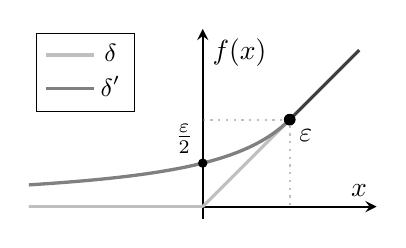
\begin{tikzpicture}
        \begin{axis}[
            % Set the axis labels
            xlabel={$x$},
            ylabel={$f(x)$},
            % Set the x-axis range
            xmin=-2,
            xmax=2,
            % Set the y-axis range
            ymin=-0.1,
            ymax=2,
            % Add axis lines through origin
            axis lines=middle,
            % Set plot width and height
            width=6cm,
            height=4cm,
            %make the axis thicker,
            % Set the aspect ratio to 1
            axis equal,
            axis line style={thick},
            % remove the labels on the x and y axis (ticks). The ticks should remain, but have no labels
            xtick=\empty,
            ytick=\empty,
            % Add a grid
            grid=both,
            legend style={
                at={(0.02,0.98)},  % Position in upper left
                anchor=north west,
                draw=black,         % No border
                fill=none,         % No background
                font=\small        % Smaller font                
            },
        ]

        \addplot[
            domain=0:\eps,
            samples=10,
            color=black!25,
            very thick,
            opacity=1.0,
        ] {x};
        \addlegendentry{$\delta$}

        \addplot[
            domain=-5:\eps,
            samples=100,
            color=black!50,
            very thick,
        ]{(\eps)^2 / (-x + 2 * \eps)};
        \addlegendentry{$\delta'$}

        \addplot[
            domain=-5:0,
            samples=10,
            color=black!25,
            very thick,
            opacity=1.0
        ] {0};

        \addplot[
            domain=\eps:1.8,
            samples=10,
            color=black!75,   
            %twice as thick as the normal 'thick'
            very thick,          
        ] {x};     

        %draw a horizontal line from epsilon to 0

        \addplot[
            thick, 
            samples=10, 
            domain=0:6,
            gray, 
            opacity=0.5,
            %make it dashed
            dotted,
            name path=three
        ] coordinates {(0, \eps)(\eps,\eps)(\eps,0)};
        
        \node[circle, fill=black, inner sep=1.5pt] at (axis cs:\eps,\eps) {};
        \node[below right] at (axis cs:\eps,\eps) {$\varepsilon$};

        \node[
            circle, 
            fill=black, 
            inner sep=1.2pt
            ] at (axis cs:0,\eps / 2) {};
        \node[
            above left, 
            %make the text smaller and gray
            black 
        ] at (axis cs:0,\eps / 2) {$\frac{\varepsilon}{2}$};
    \end{axis}
    \end{tikzpicture}
    \caption{Comparing the standard ($\delta$) and decaying ($\delta'$) penetration depth functions.}
    \label{plot:penetration_base_decay}
\end{figure}
